% Adapted layer styles from haiyichen001/tikz-figure-skill transformer.tex (MIT),
% revision 5952e18631600aa46de91ea7653f92ae6697d774. New generic pre-norm topology.
% This is an abstract conditioned Transformer block, NOT an exact DiT/SD3/Flux implementation.
\documentclass[tikz,border=10pt]{standalone}
\usepackage{amsmath,amssymb}
\usetikzlibrary{positioning,arrows.meta,calc}
\definecolor{acaBlueLine}{HTML}{6080B0}\definecolor{acaBlueFill}{HTML}{DBEAFE}
\definecolor{acaGreenLine}{HTML}{308568}\definecolor{acaGreenFill}{HTML}{D7EBDF}
\definecolor{acaOrangeLine}{HTML}{B87930}\definecolor{acaOrangeFill}{HTML}{FFE6CC}
\definecolor{acaPurpleLine}{HTML}{87639C}\definecolor{acaPurpleFill}{HTML}{EDE3F2}
\def\rowSep{1.05}\def\conditionText{Time $t$ and condition $c$}
\begin{document}
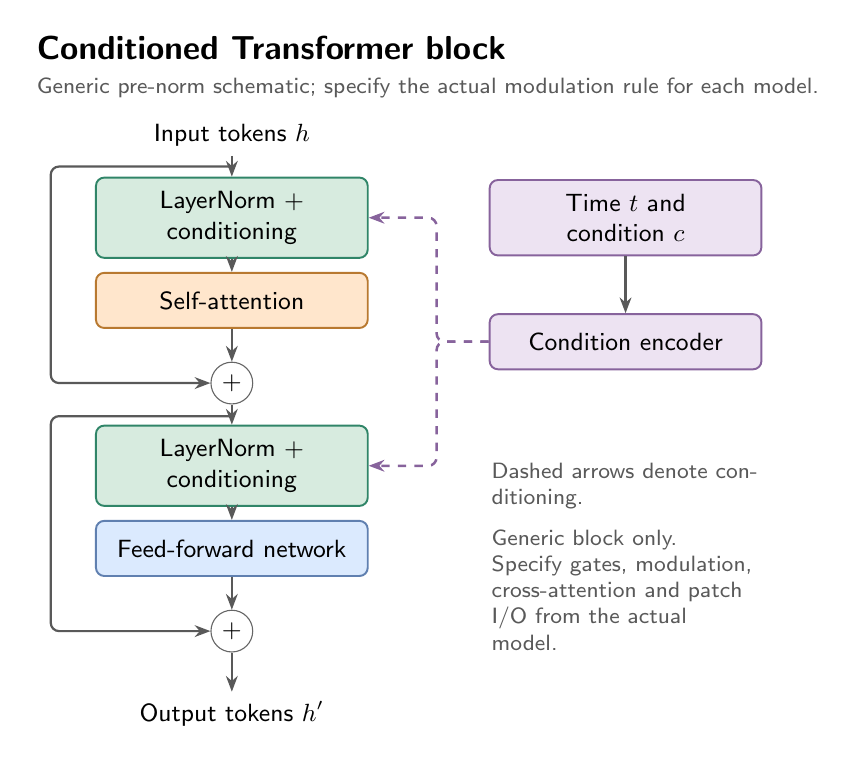
\begin{tikzpicture}[>={Stealth[length=2mm]},font=\sffamily\small,
 layer/.style={draw,line width=.7pt,rounded corners=3pt,text width=3.1cm,align=center,minimum height=.70cm,inner sep=5pt},
 norm/.style={layer,fill=acaGreenFill,draw=acaGreenLine},
 attn/.style={layer,fill=acaOrangeFill,draw=acaOrangeLine},
 ffn/.style={layer,fill=acaBlueFill,draw=acaBlueLine},
 cond/.style={layer,fill=acaPurpleFill,draw=acaPurpleLine},
 sum/.style={circle,draw=black!60,fill=white,inner sep=2pt,minimum size=.45cm},
 flow/.style={->,line width=.8pt,draw=black!65},
 branch/.style={flow,rounded corners=3pt},
 conditioning/.style={->,line width=.9pt,draw=acaPurpleLine,dashed,rounded corners=3pt}]
\node[font=\sffamily\bfseries\large,anchor=west] at (-2.6,1.1) {Conditioned Transformer block};
\node[font=\sffamily\footnotesize,text=black!65,anchor=west] at (-2.6,.60) {Generic pre-norm schematic; specify the actual modulation rule for each model.};
\node (input) at (0,0) {Input tokens $h$};
\node[norm] (norm_attn) at (0,-\rowSep) {LayerNorm + conditioning};
\node[attn] (attention) at (0,-2*\rowSep) {Self-attention};
\node[sum] (add_attn) at (0,-3*\rowSep) {$+$};
\node[norm] (norm_ffn) at (0,-4*\rowSep) {LayerNorm + conditioning};
\node[ffn] (feed_forward) at (0,-5*\rowSep) {Feed-forward network};
\node[sum] (add_ffn) at (0,-6*\rowSep) {$+$};
\node (output) at (0,-7*\rowSep) {Output tokens $h'$};
\node[cond] (condition) at (5,-\rowSep) {\conditionText};
\node[cond] (mapper) at (5,-2.5*\rowSep) {Condition encoder};
\draw[flow] (condition)--(mapper);
\foreach \a/\b in {input/norm_attn,norm_attn/attention,attention/add_attn,add_attn/norm_ffn,norm_ffn/feed_forward,feed_forward/add_ffn,add_ffn/output}
 \draw[flow] (\a.south)--(\b.north);
\draw[branch] (0,-.4) -- (-2.3,-.4) |- (add_attn.west);
\draw[branch] (0,-3.4*\rowSep) -- (-2.3,-3.4*\rowSep) |- (add_ffn.west);
\draw[conditioning] (mapper.west) -- (2.6,-2.5*\rowSep) |- (norm_attn.east);
\draw[conditioning] (mapper.west) -- (2.6,-2.5*\rowSep) |- (norm_ffn.east);
\node[align=left,text width=3.4cm,font=\sffamily\footnotesize,text=black!65] at (5,-5.1*\rowSep) {Dashed arrows denote conditioning.\\[5pt]Generic block only.\\Specify gates, modulation,\\cross-attention and patch\\I/O from the actual model.};
\end{tikzpicture}
\end{document}
